%%%%%%%%%%%%%%%%%%%%%%%%%%%%%%%%%%%%%%%%%%%%%%%%%%%%%%
%
% Where we describe the simulation systems and frameworks that are
% needed for the DUNE experiment ranging from generation to detector
% response and simulation.
%%%%%%%%%%%%%%%%%%%%%%%%%%%%%%%%%%%%%%%%%%%%%%%%%%%%%%
\chapter{Simulation Systems and Frameworks}  %% Tom Junk lead editor
 \fixme{10 pages}
%%%%%%%%%%%%%%%%%%%%%%%%%%%%%%%%%%%%%%%%%%%%%%%%%%%%%%
\section{Beam simulation Systems}

%%%%%%%%%%%%%%%%%%%%%%%%%%%%%%%
\subsection{G4LBNF}

\subsection{Beam Spectrometer Simulation}

\subsection{Muon Monitors}

%%%%%%%%%%%%%%%%%%%%%%%%%%%%%%%%%%%%%%%%%%%%%%%%%%%%%%
\section{Event Generators}

Event generators play a critical role in neutrino experiments and should receive the 
same level of attention as paid to the experimental apparatus. 
A generator must simulate all the details of every particle that appears in the final state on an event-by-event basis.
The event generators provided with LArSoft create MCParticle and MCTruth data products in
the {\it{art}} event store.  Any number of event generators, including multiple instances of the
same generator, may be run for a given event.  This feature is useful in order to overlay cosmic
rays and radiological decays on neutrino scattering events for example.  In addition to the
generators listed below that are integrated into the LArSoft software environment, a text-file generator
can read files with particle types and four-vectors of their momenta and energies to provide access
to additional generators without investing in software integration.

%%%%%%%%%%%%%%%%%%%%%%%%%%%%%%%%%%%%%%%%%%%%%%%%%%%%%%
\subsection{Neutrino Interaction simulations}

An ideal input theory of neutrino-nucleus interactions
 would provide internally consistent and fully-differential cross sections 
in the kinematics of every final-state particle, over all reaction mechanisms, over the full energy range, for all combinations of neutrino flavor and helicity, and for every nucleus in the experiment.
However, modern theory generally provides only the kinematics for the final state lepton, with minimal guidance on the hadronic side, and only for a subset of the experimentally accessible phase space.
Thus, as implemented in event generators, neutrino-nucleus interactions are factorized as a ``product'' of a free nucleon scattering, a ground state nuclear model, hadronization, and hadron transport (and decay).

%%%%%%%%%%%%%%%%%%%%%%%%%%%%%%%
\subsubsection{GENIE $\nu$ interaction generator}

GENIE (Generates Events for Neutrino Interaction Experiments) \cite{Andreopoulos:2009rq} is the most widely-used event generator in neutrino experiments today.
It is a core component of the software stack for every running and planned neutrino beam experiment in the United States.
In accelerator neutrino experiments, observables are a convolution of the flux, interaction physics, and detector response. 
Three corresponding pieces combine to form the software stack, as illustrated in Figure \ref{fig:3partstack}.
Event generators sit at the heart of the stack and provide experimenters with access to the physics of the neutrino interaction. GENIE is the primary generator for 
ArgoNeuT \cite{Anderson:2012vc}, 
DUNE \cite{Acciarri:2015uup}, 
MicroBooNE \cite{Fleming:2012gvl}, 
MIER$\nu$A \cite{MINERvA:2006aa}, 
NO$\nu$A \cite{Ayres:2007tu}, 
and SBND \cite{Antonello:2015lea,sbnd}, 
because of its flexible framework and fully-featured geometry and flux drivers.

\begin{figure}
  \centering
  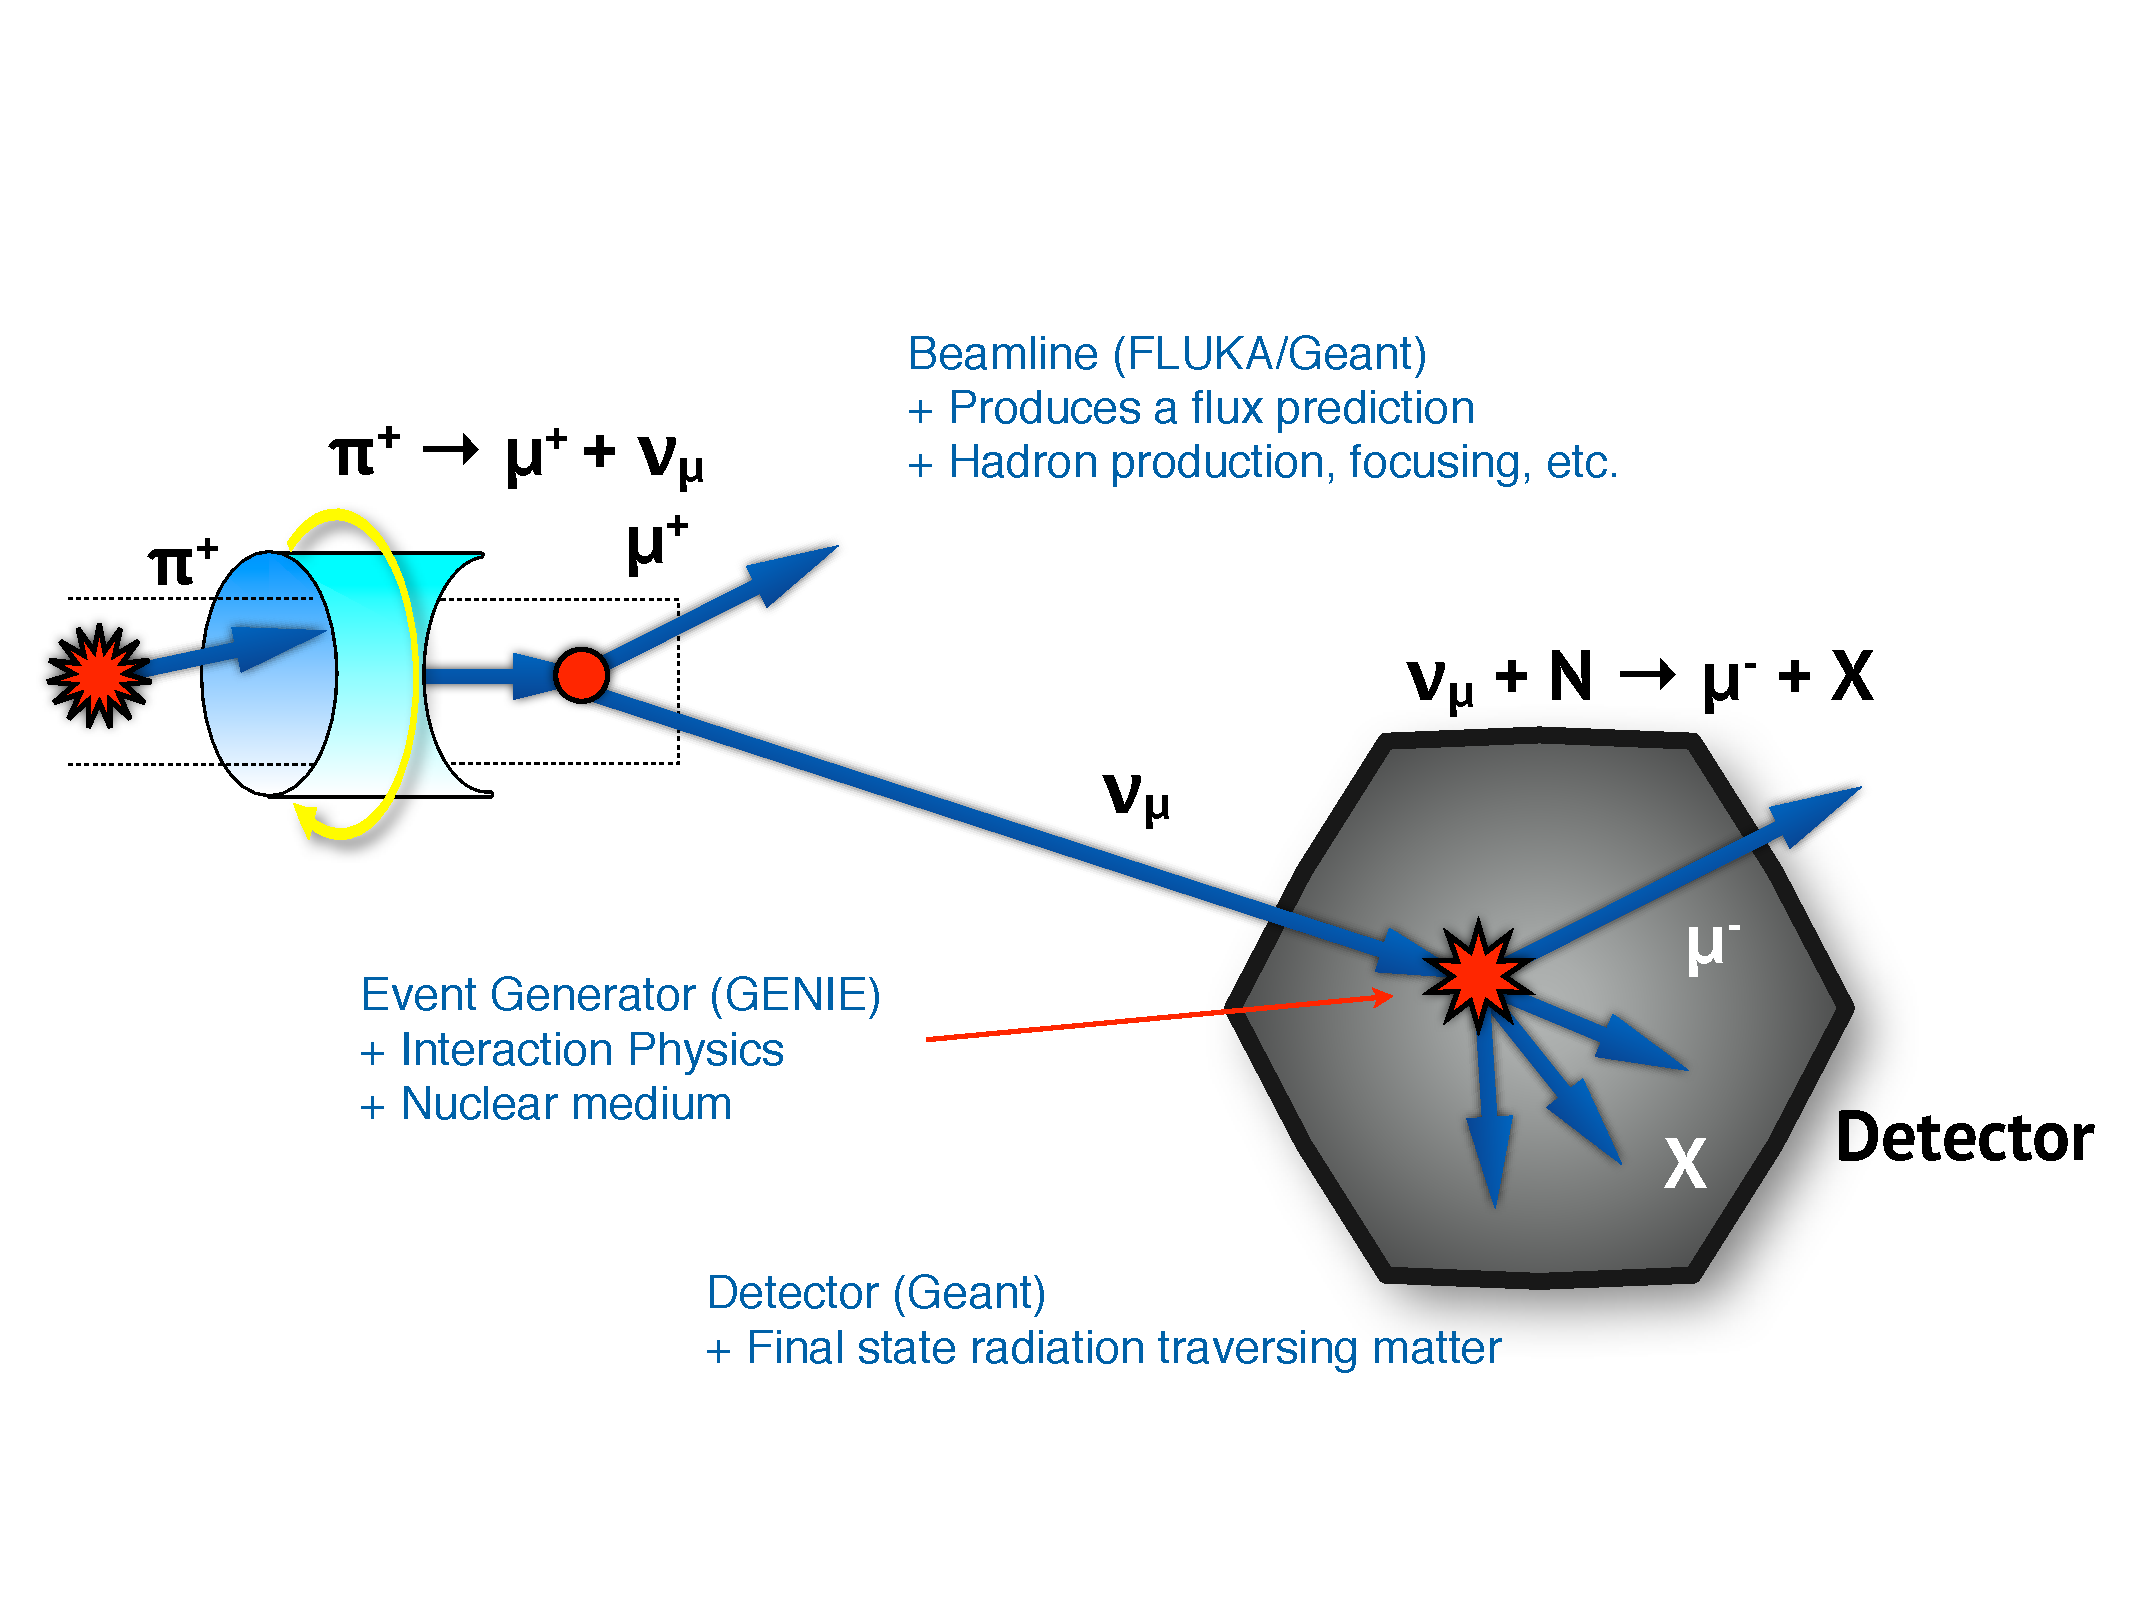
\includegraphics[height=0.32\textheight]{software-computing/figures/3partstack}
  \caption{The accelerator neutrino experiment software stack. Figure provided by G. N. Perdue.}
  \label{fig:3partstack}
\end{figure}

Neutrino experiments observe final state particle spectra, after transport through the dense nuclear medium.
Relating these observable quantities to the true, underlying kinematics is only possible through a model, as implemented through an event generator.
Experiments use event generators to connect observed event topologies to the true underlying kinematics.
At best we may build a map, weighted by probability, that links all possible initial states to an observed final state.
With this map, we may infer a probabilistic neutrino energy distribution (or a different kinematic distribution).

GENIE provides a rich toolkit to its users:
\begin{itemize}
\item a geometry engine for modeling complex detectors (compatible with a Geant detector definition),
\item flux drivers for computing exposure (atmospheric/solar sources) and normalizing responses to accelerator beams,
\item event re-weighting engines for systematic uncertainties and error propagation,
\item databases of electron, hadron, and neutrino scattering results with applications for comparing simulation and data,
\item electron and hadron scattering event generator functionality,
\item nucleon decay generators, and
\item libraries of pre-computed cross sections.
\end{itemize}

The GENIE global physics model is built from a collection of exclusive state models (e.g., Llewellyn Smith QE, Rein-Sehgal resonant pion production, Bodek-Yang DIS, etc.).
(Many of these are wrong but useful.) 
When a new process is added (e.g., Nieves group MEC), it is necessary to retune the total cross section by controlling the strength of all the various exclusive processes to keep GENIE generally consistent with data for the total cross section.

GENIE contains dozens of different physics models.
The default nuclear model is the relativistic Fermi gas with Bodek and Ritchie corrections (to model high-momentum tails).
GENIE also implements the Effective Spectral Function, and the Local Fermi Gas.
Other spectral function implementations exist in development branches.
The quasielastic process defaults to Llewellyn-Smith, but GENIE also contains the Nieves et al model. 
The axial form factor model is the dipole but the z-expansion model is available as well.
Excitation of nucleon resonances (decaying by meson emission) and coherent pion production are both described by default by models by Rein and Sehgal, but there are a number of alternatives (Berger and Sehgal, different form factor models, etc.).
GENIE also contains a diffractive pion production model (Rein), but it is not activated by default.
Models for neutrino-electron scattering and inverse muon decay are included and are mostly complete - additional radiative corrections required for neutrino-electron scattering.

GENIE also offers a custom built and the Valencia ``2p2h'' models.
Bodek and Yang (2003) is used for non-resonant inelastic scattering.
Other interesting exclusive states (e.g., QEL hyperon production, single Kaon production, etc.) are optional (to avoid double counting in the hadronization model).
The custom ``AGKY'' hadronization model covers a transition between PYTHIA at high ($W > 3$ GeV/c$^2$) invariant masses and an empirical model based on KNO-scaling at lower $W$.
GENIE has two internally developed models for final-state interactions; one is a cascade model and the other (the default) parameterizes the cascade a single effective interaction for fast and simple re-weighting.
GENIE uses the SKAT parametrization of formation zones (the effective distance over which a quark hadronizes).


%%%%%%%%%%%%%%%%%%%%%%%%%%%%%%%
\subsubsection{NEUT $\nu$ interaction generator}

%%%%%%%%%%%%%%%%%%%%%%%%%%%%%%%
\subsubsection{NuWro $\nu$ interaction generator}

%%%%%%%%%%%%%%%%%%%%%%%%%%%%%%%
\subsubsection{NUANCE $\nu$ interaction generator}

%%%%%%%%%%%%%%%%%%%%%%%%%%%%%%%
\subsubsection{GIBUU $\nu$ interaction generator}

%%%%%%%%%%%%%%%%%%%%%%%%%%%%%%%
\subsubsection{MARLEY $\nu$ interaction generator}

%%%%%%%%%%%%%%%%%%%%%%%%%%%%%%%%%%%%%%%%%%%%%%%%%%%%%%
\subsection{Nucleon Decay and Exotic Particle Simulation}

The nucleons in $^{40}Ar$ nuclei are bound together very tightly, and have nonzero expectation values of their
kinetic energies.  When a nucleon decays, the decay products scatter within the nucleus before exiting, in a manner
similar to scattering products in neutrino interactions.  The resulting nucleus de-excites into a stable configuration
after the event.  Nucleon-decay generators take these effects into account.  Similar issues exist for neutron-antineutron
oscillaton signal models.

 
%%%%%%%%%%%%%%%%%%%%%%%%%%%%%%%
\subsubsection{GENIE}  % Hector Mendez will supply something here.

%%%%%%%%%%%%%%%%%%%%%%%%%%%%%%%
\subsubsection{MadGraph/MadEvent}

\subsection{Cosmic-Ray Generators}

While the Far Detector is 4850 feet underneath the surface and thus has a low rate of cosmic rays (approximately 
four per day per m$^2$ penetrate the top surface), these cosmic-ray events contribute significantly to the data
volume and they are quite useful for calibrating the detector.  Their energies are quite high; the average energy
of a cosmic-ray muon at the 4850-foot level is approximately 400~GeV.  Many of the cosmic-ray muons will produce
electromagnetic showers in the detector, while others will be present as minimum-ionizing particles, or populate
the relativistic rise portion of the Bethe-Bloch curve.  Careful simulation of cosmic-ray events will be necessary
to take advantage of them for calibration purposes, as well as to identify them as backgrounds to physics analyses
such as atmospheric-neutrino measurements and nucleon-decay searches.

%%%%%%%%%%%%%%%%%%%%%%%%%%%%%%%
\subsubsection{CRY}

%%%%%%%%%%%%%%%%%%%%%%%%%%%%%%%
\subsubsection{CORSIKA}

%%%%%%%%%%%%%%%%%%%%%%%%%%%%%%%
\subsubsection{MUSUN/MUSIC}  % from Karl and Vitaly

The MUSUN (MUon Simulations UNderground) event generator is described in Refs~\cite{Kudryavtsev:2008qh}
and~\cite{Kudryavtsev:2003aua}.
It uses the results of muon transport through rock using 
MUSIC (Muon SImulation Code)~\cite{Antonioli:1997qw,Kudryavtsev:1999zu,Kudryavtsev:2008qh}
convolved with the muon spectrum at sea level for different zenith angles. 
MUSUN, originally a Fortran program, has been rewritten in C++ and integrated into LArSoft.
The MUSUN code, as currently adapted for DUNE, samples muons around an 
underground laboratory located near the Ross shaft, with a latitude of
44$^\circ$~20$^\prime$~45.21$^{\prime\prime}$~N, and a longitude of
103$^\circ$~45$^\prime$~161$^{\prime\prime}$~W. The rock composition has been
taken from Refs.~\cite{Mei:2009py} and~\cite{ref:ZhaoPrivateCommunication1}. 
In the MUSIC simulation for SURF, the rock is assumed to be uniform
with average properties derived from many samples taken at the laboratory. 
The composition of the rock in the simulation correspons to
$\langle Z\rangle = 12.09$ and $\langle A\rangle = 24.17$~\cite{Mei:2009py,ref:ZhaoPrivateCommunication1}, with
an average density of 2.70 g/cm$^{3}$~\cite{ref:ZhaoPrivateCommunication1}.
Other measurements suggest that the density may be larger (2.8-2.9 g/cm$^{3}$~\cite{Gray:2010nc,Heise:2014gta}). The
density can be changed in the MUSUN muon generator if required. The slant depth 
distribution for the 4850~ft level at SURF was calculated from the CGIAR digital elevation
model~\cite{ref:MartinRichardsonThesis}.
The measurement of the muon flux at SURF (in the Davis campus near the Yates shaft)
was performed by the active veto system of the Davis experiment~\cite{Cherry:1983dp} giving the value of
($5.38\pm0.07)\times10^{-9}$ cm$^{-2}$~s$^{-1}$~sr$^{-1}$ for the vertical flux.  
The measured fraction of multiple
muons has been added to the single muon flux as given in Ref.~\cite{Cherry:1983dp}, so the systematic
uncertainty for this value may be of the order of a few percent. MUSIC/MUSUN predicts
$5.18\times10^{-9}$~cm$^{-2}$~s$^{-1}$~sr$^{-1}$ at the Davis campus, in agreement with
the measurement. A recent measurement of muons in the Davis campus has been
carried out with the active veto system of the Majorana demonstrator~\cite{Abgrall:2016cfi} giving the
value of $5.31\pm0.17\times10^{-9}$~cm$^{-2}$~s$^{-1}$ for the total (not vertical) muon flux, in reasonable
agreement with a calculation with MUSIC/MUSUN for a close location, also in the Davis
campus but LUX/LZ location rather than Majorana demonstrator hall:
$6.16\times10^{-9}$~cm$^{-2}$~s$^{-1}$.   The systematic uncertainty in the muon flux prediction
is estimated to be 20\%.  An accurate measurement of the muon flux in the DUNE caverns
is required to normalize simulations.

The total muon flux through a sphere with unit cross-sectional area is calculated as $5.66\times
10^{-9}$~cm$^{-2}$~s$^{-1}$ and the mean muon energy is 283~GeV.
The normalisation of the muon flux or rate is done for a specic point underground where
the slant depth distribution was calculated, assuming that the muon flux is the same 
everywhere in the cavern and also in the
rock where the box for muon sampling is extended. For the cavern(s) where the far
detector will be located the difference in muon intensities in different locations is not
expected to exceed 10%.
In the MUSUN generator for DUNE, muons are sampled on a surface of a box that
encompasses the lab and a few metres of rock around the cavern. The rock is 
included to make sure that muon-induced cascades initiated above and around the cavern
have enough space to fully develop and produce secondaries that may enter the active volume
of the detector even if the primary muon does not.
The size of the box is $74.43\times29.54\times30.18$ m$^{3}$. The size of
the cryostat has been assumed to be $61.62\times14.94\times13.58$~m$^{3}$.
Muons are sampled according to their energy spectrum for a particular zenith and 
azimuthal angles, sampled in turn from the angular distribution obtained using MUSIC. 
The size of the box (the probability of a muon to cross a particular
surface of the box) is taken into account when generating muons. All energy spectra 
and angular distributions are stored on disk and read during the initialization at
the beginning of each simulation run. 

The muon rate through the surface of this box is $0.1579\pm 0.0316$~Hz. This rate can be used
to normalise cosmic-ray simulations in DUNE. The rate of muons passing through
the active volume of liquid argon with a minimum track length of 1~m 
is $0.053\pm 0.011$~Hz, or about about 30% of muons generated on the
surface of the box.


%%%%%%%%%%%%%%%%%%%%%%%%%%%%%%%
\subsection{Radiological Generator}

The radiological generator is a LArSoft module that produces MCParticle objects corresponding
to the decay products of radionuclides.  The spectra of alpha, beta, and gamma particles emitted
by decaying radionuclides are user-specifialbe in root files.  The radiological generator generates
decays within a rectangular prism in space and in a specified range of time.  For a particular
nuclide, volumes in the geometry whose materials match a regular expression are selected as locations
for possible decays.  This mechanism is chosen over the more complex alternatie of specifying radionuclide
concentrations in the geometry specification because GEANT4 and GENIE will attempt to simulate interactions
of neutrinos and other particles on extremely rare nuclides, for which cross-section data may not exist.
The CPU time required to run the radiological generator is negligible, but its output can dominate
the CPU and storage of the fully simulated samples, as is the case for the far detector data.

%%%%%%%%%%%%%%%%%%%%%%%%%%%%%%%%%%%%%%%%%%%%%%%%%%%%%%
\section{Detector geometry and modeling systems}

LArSoft reads in GDML files that describe the geometries of the far detector modules.  Two versions of these
files are required -- one with the readout wires described, and one without.  The total mass in the readout
wires is very small, but their presence would increase the memory and CPU requirements of the simulation
if they are present in any more than a parameterized manner.  These GDML files are constructed with Perl scripts.
A more sophisticated tool called {\tt{ggd}}~\cite{ref:ggd} is designed to create GDML files from a higher-level
Python description of the detector.

Within LArSoft, two ``parallel-world'' representations of the geometry are created.  One is for particle interactions
modeled by GEANT4, and the other is intended for GEANT4's simulation of photon propagation.

%%%%%%%%%%%%%%%%%%%%%%%%%%%%%%%
\subsection{Fast Monte Carlo}

A Fast Monte Carlo (FMC) program was developed by the LBNE collaboration and was used to
compute oscillation sensitivities~\cite{Acciarri:2015uup}.  The FMC simulated neutrino interactions
on argon using the LBNF flux spectrum and the GENIE~\cite{Andreopoulos:2009rq} generator.  The detector
responses to the final-state particles produced by GENIE are approximated with efficiency
fractions as functions of particle energy, energy resolution smearing fractions, and
correct and incorrect particle identification rates.  The events were divided into
$\nu_\mu$CC-like, $\nu_e$-CC-like, and NC-like, for the near and far detectors, and the
inputs provided to a parameter fit, such as CAFANA, GLoBES, or LOAF.  The details of the
detector response and analysis requirements can be found in~\cite{Acciarri:2015uup}.  The CPU time needed
for the FMC project is 1 to 4~M hours per year, with $<1$~TB of storage required, when
it is fully used.  The emphasis on full simulation and reconstruction results however has
displaced the FMC in 2016 and 2017. 

%%%%%%%%%%%%%%%%%%%%%%%%%%%%%%%
\subsection{Geant4 and Detector Response Modeling}

Interactions of particles with the detector materials, both active and inactive, is simulated with 
GEANT4~\cite{geant4,Allison:2006ve}.  GEANT4 is also used as the underlying physics model for G4LBNF, the
simulation of the baffle, target, horns, and decay pipe.  GEANT4 simulates particle trajectories in steps,
taking into account electric and magnetic fields, as well as interaction and scattering probabilities in the
matter at each step.  GEANT4 requires a detailed description of the geometry of the materials through which
it simulates particle propagation.

LArSoft~\cite{larsoft.org} provides an interface to GEANT4 that is optimized for liquid argon time projection
chambers.  Step sizes are limited by voxelizing the active liquid argon volume into cubes 300~$\mu$m on a side.
Ionization and scintillation are modeled with a modified box function~\cite{Thomas:1987zz} or with 
NEST~\cite{Szydagis:2011tk,Szydagis:2013sih,Mock:2013ila,Lenardo:2014cva}, using
the energy deposition on each step provided by GEANT4.  Ionization and delta rays are part of a continuous
spectrum -- GEANT4 tracks delta rays down to an energy of ??~KeV using the default LArSoft paramaterization.
The GEANT4 step of a LArSoft simulation typically runs as a separate job, and the output of this job is the
number of electrons deposited on each wire after LArSoft's custom drift and diffusion simulation, which
takes into account recombination, electron lifetime, space charge, and detector geometry effects.  The charge
is summed over all contributing particle steps and integrated over diffusion, and reported separately for
each particle for each tick on each wire (a particle may have many small GEANT4 steps which contribute
charge to a wire).  The average position of the charge creation points are recorded for each particle for each
tick on each wire as well.  

In the LArSoft interface,  it is possible to specify a magnetic field that will cause charged-particle
trajectories to deflect.

For photon propagation modeling, a library-based method is used to speed up the sampling of tens of thousands of
scintillation photons per MeV of deposited energy.  The photon library is a list of detection probabilities
indexed by the voxel in space corresponding to the origin of the photons and the photon detector channel.
The source voxel sizes are cubes ??~cm on a side.  These detection probabilites are computed with a fully-simulated
run using GEANT4 to propagate photons isotropically-distributed in their production angle through the liquid argon,
taking into account the reflectivity of the field cage walls and the cathode and Rayleigh scattering in the liquid.
The detection probability further includes light attenuation along the length of each photon detector's bar.  An
overall quantum efficiency scaling factor is applied before the photon library lookup is performed, reducing the
number of lookups needed to complete the calculation.  The photon lookup library is typically a 300~MB rootfile.
Cherenkov radiation is currently not simulated or propagated by LArSoft; it may be added in a future version.

The GEANT4 step, along with the LArSoft-supplied drift modeling and lookup-library-based photon propagation, 
is the second-quickest simulation step,
after the generation stage, with ??~sec/event for far detector neutrino interactions, and ??~sec/event for
ProtoDUNE events with cosmic rays.  GEANT4 however requires several GB of auxiliary data files in order
to parameterize the interactions of particles with matter.  The GEANT4 collaboration actively compares
the modeling of published data distributions and tunes the simulation to improve the modeling.

%%%%%%%%%%%%%%%%%%%%%%%%%%%%%%%
\subsection{GeantV}

%%%%%%%%%%%%%%%%%%%%%%%%%%%%%%%%%%%%%%%%%%%%%%%%%%%%%%
\section{FLUKA}

FLUKA~\cite{Bohlen:2014buj,Ferrari:2005zk} is a full-featured physics and detector simulation package.  It is capable of
performing the same role as GEANT4 in the beam simulations, as well as in the detector response modeling.
FLUKA also has the ability to model neutrino-nucleus interactions, and thus can substitute for GENIE.
Due to the prohibitive computational load of simulating all of the drifting electrons and propagating
photons, the same solution of a custom LArSoft-based drift and charge deposit model would still be needed
if FLUKA were to take on all other roles.  A project has started to interface FLUKA at several points upstream
of the detector charge deposit modeling.  Comparing FLUKA-based calculations with those based on GEANT4 and
GENIE provides additional abilities to model external data and detector data properly, and to estimate
systematic uncertainties.

%%%%%%%%%%%%%%%%%%%%%%%%%%%%%%%%%%%%%%%%%%%%%%%%%%%%%%
\section{Electronics and DAQ Emulation}

The output of the GEANT4 step, which consists of simulated charge deposits on each wire, requires
additional processing to model the expected signals to be digitized.  The digitizers measure the
current on each wire integrated over the sampling time, chosen to be 2~$\mu$s.  As charge drifts
by an induction-plane wire, it induces a current that is a bipolar function of time, while the
current in a collection-plane wire is a unipolar function of time.  The differences in the arrival
times of charge drifting past the layers due to the finite spacing between the layers are include.
LArSoft parameterizes the response
of the detector as a Green's function -- the response of a packet of charge localized in space and time,
and this funtion is convoluted with the function describing the arrival times of the charges passing by
or collecting on the wires.  This convolution is performed in frequency space after FFT'ing the charge
arrival function.  At this stage, the electronics response transfer function is multiplied in.  An inverse
FFT predicts the time-domain signal.  The signal gain is a separately controllable parameter in LArSoft.
  Noise is then added, either white noise or an exponentially falling
spectrum, and then the result is discretized and truncated to the expected range of the 12-bit ADCs.  

Additional steps, such as modeling of stuck bits or groups of bits are configurable within LArSoft.
Modeling dead channels or groups of channels is frequently performed as an early step
in the reconstruction job so that Monte Carlo samples can be reused with varying fractions and placement
of dead channels.

Similar processing steps are applied to the simulation of the photon detector waveforms.

The output of the electronics simulation is digitized waveforms.  Zero suppression is optionally
applied.  The simulated data are compressed either with ROOT's built-in compression, or a fixed-dictionary
Huffman algorithm.

%%%%%%%%%%%%%%%%%%%%%%%%%%%%%%%%%%%%%%%%%%%%%%%%%%%%%%
\section{Trigger Simulation}

Triggers are being designed for the Far Detector, and the tradeoffs between physics sensitivity,
trigger rate, buffer size, and data volume are investigated with simulated signal events and
realistic backgrounds.  Cosmic-ray events, beam-neutrino interactions, atmospheric neutrino interations,
and nucleon decay events are the easiest to trigger on, using energy-sum triggers.  These events
are also confined to a very short amount of time, and so readout of the detector for a drift time plus some
extra before and after to capture pedestals is expected to suffice.
 
 Supernova-burst triggers on the other hand pose significant challenges.  The burst of neutrinos is expected
to last tens of seconds, in which a few tens to a few thousands of neutrino scatters may be recorded.  The
triggering system must identify a burst quickly in order to save full detector information in a buffer
long enough to capture the entire burst.  Disk-writing speeds and network speeds will not be fast enough
to save an entire burst, though SSD's may provide sufficient write speed.  A trigger must be formed so 
as not to write over the SSD memory continuously.  This trigger needs to run on specialized hardware, and/or
computers dedicated to triggering supernova events, possibly with GPU assistance.  As such, LArSoft is
unlikely to be the right tool for computing trigger decisions, but LArSoft-simulated MC samples are
ideal for providing input to smaller, faster trigger algorithms developed separately.
